% Class 1 — Seeing Data. Build: lualatex seeing-data.tex (run twice).
\documentclass[aspectratio=169,11pt]{beamer}

\usepackage{graphicx}
\usepackage{booktabs}
\graphicspath{{figs/}}

% ---- course look: charcoal ground, coral accent ----
\definecolor{ink}{HTML}{F5F1E8}
\definecolor{ground}{HTML}{23272B}
\definecolor{coral}{HTML}{FF6B5A}
\definecolor{mist}{HTML}{9AA3AB}

\usetheme{default}
\usefonttheme{professionalfonts}
\renewcommand{\familydefault}{\sfdefault}
\setbeamertemplate{navigation symbols}{}
\setbeamercolor{background canvas}{bg=ground}
\setbeamercolor{normal text}{fg=ink}
\setbeamercolor{frametitle}{fg=ink}
\setbeamercolor{structure}{fg=coral}
\setbeamercolor{alerted text}{fg=coral}
\setbeamertemplate{itemize item}{\color{coral}\rule[0.45ex]{0.6em}{0.12em}}
\setbeamertemplate{itemize subitem}{\color{mist}\rule[0.45ex]{0.4em}{0.12em}}
\setbeamertemplate{frametitle}{%
  \vspace*{1.1em}%
  {\color{mist}\scriptsize\MakeUppercase{\insertframesubtitle}}\\[0.15em]
  {\LARGE\bfseries\insertframetitle}\\[0.2em]
  {\color{coral}\rule{3em}{0.18em}}%
}
\setbeamertemplate{footline}{%
  \hspace*{1.5em}{\color{mist}\tiny 36104 · Class 1 · Seeing Data}\hfill
  {\color{mist}\tiny\insertframenumber}\hspace*{1.5em}\vspace*{0.8em}}

\newcommand{\kicker}[2]{% big section-break slide
  \begin{frame}[plain]\begin{center}
    \vspace*{\fill}
    {\color{coral}\bfseries\scriptsize\MakeUppercase{#1}}\\[0.6em]
    {\Huge\bfseries #2}
    \vspace*{\fill}
  \end{center}\end{frame}}
\newcommand{\credit}[1]{{\color{mist}\tiny #1}}

\title{Seeing Data}
\author{36104 Data Visualisation and Narratives}

\begin{document}

% ---------- 1 · title ----------
\begin{frame}[plain]
  \vspace*{\fill}
  {\color{coral}\bfseries\scriptsize 36104 · CLASS 1}\\[0.6em]
  {\fontsize{34}{38}\selectfont\bfseries Seeing Data}\\[0.5em]
  {\Large\color{mist} Visualisation, intelligence, and interpretation}\\[2em]
  {\small How do charts create meaning?}
  \vspace*{\fill}
\end{frame}

% ---------- 2 · silent chart reading ----------
\begin{frame}[t]{Before anything is explained}\framesubtitle{Silent chart reading · 5 minutes}
  \begin{columns}[T]
    \begin{column}{0.62\textwidth}
      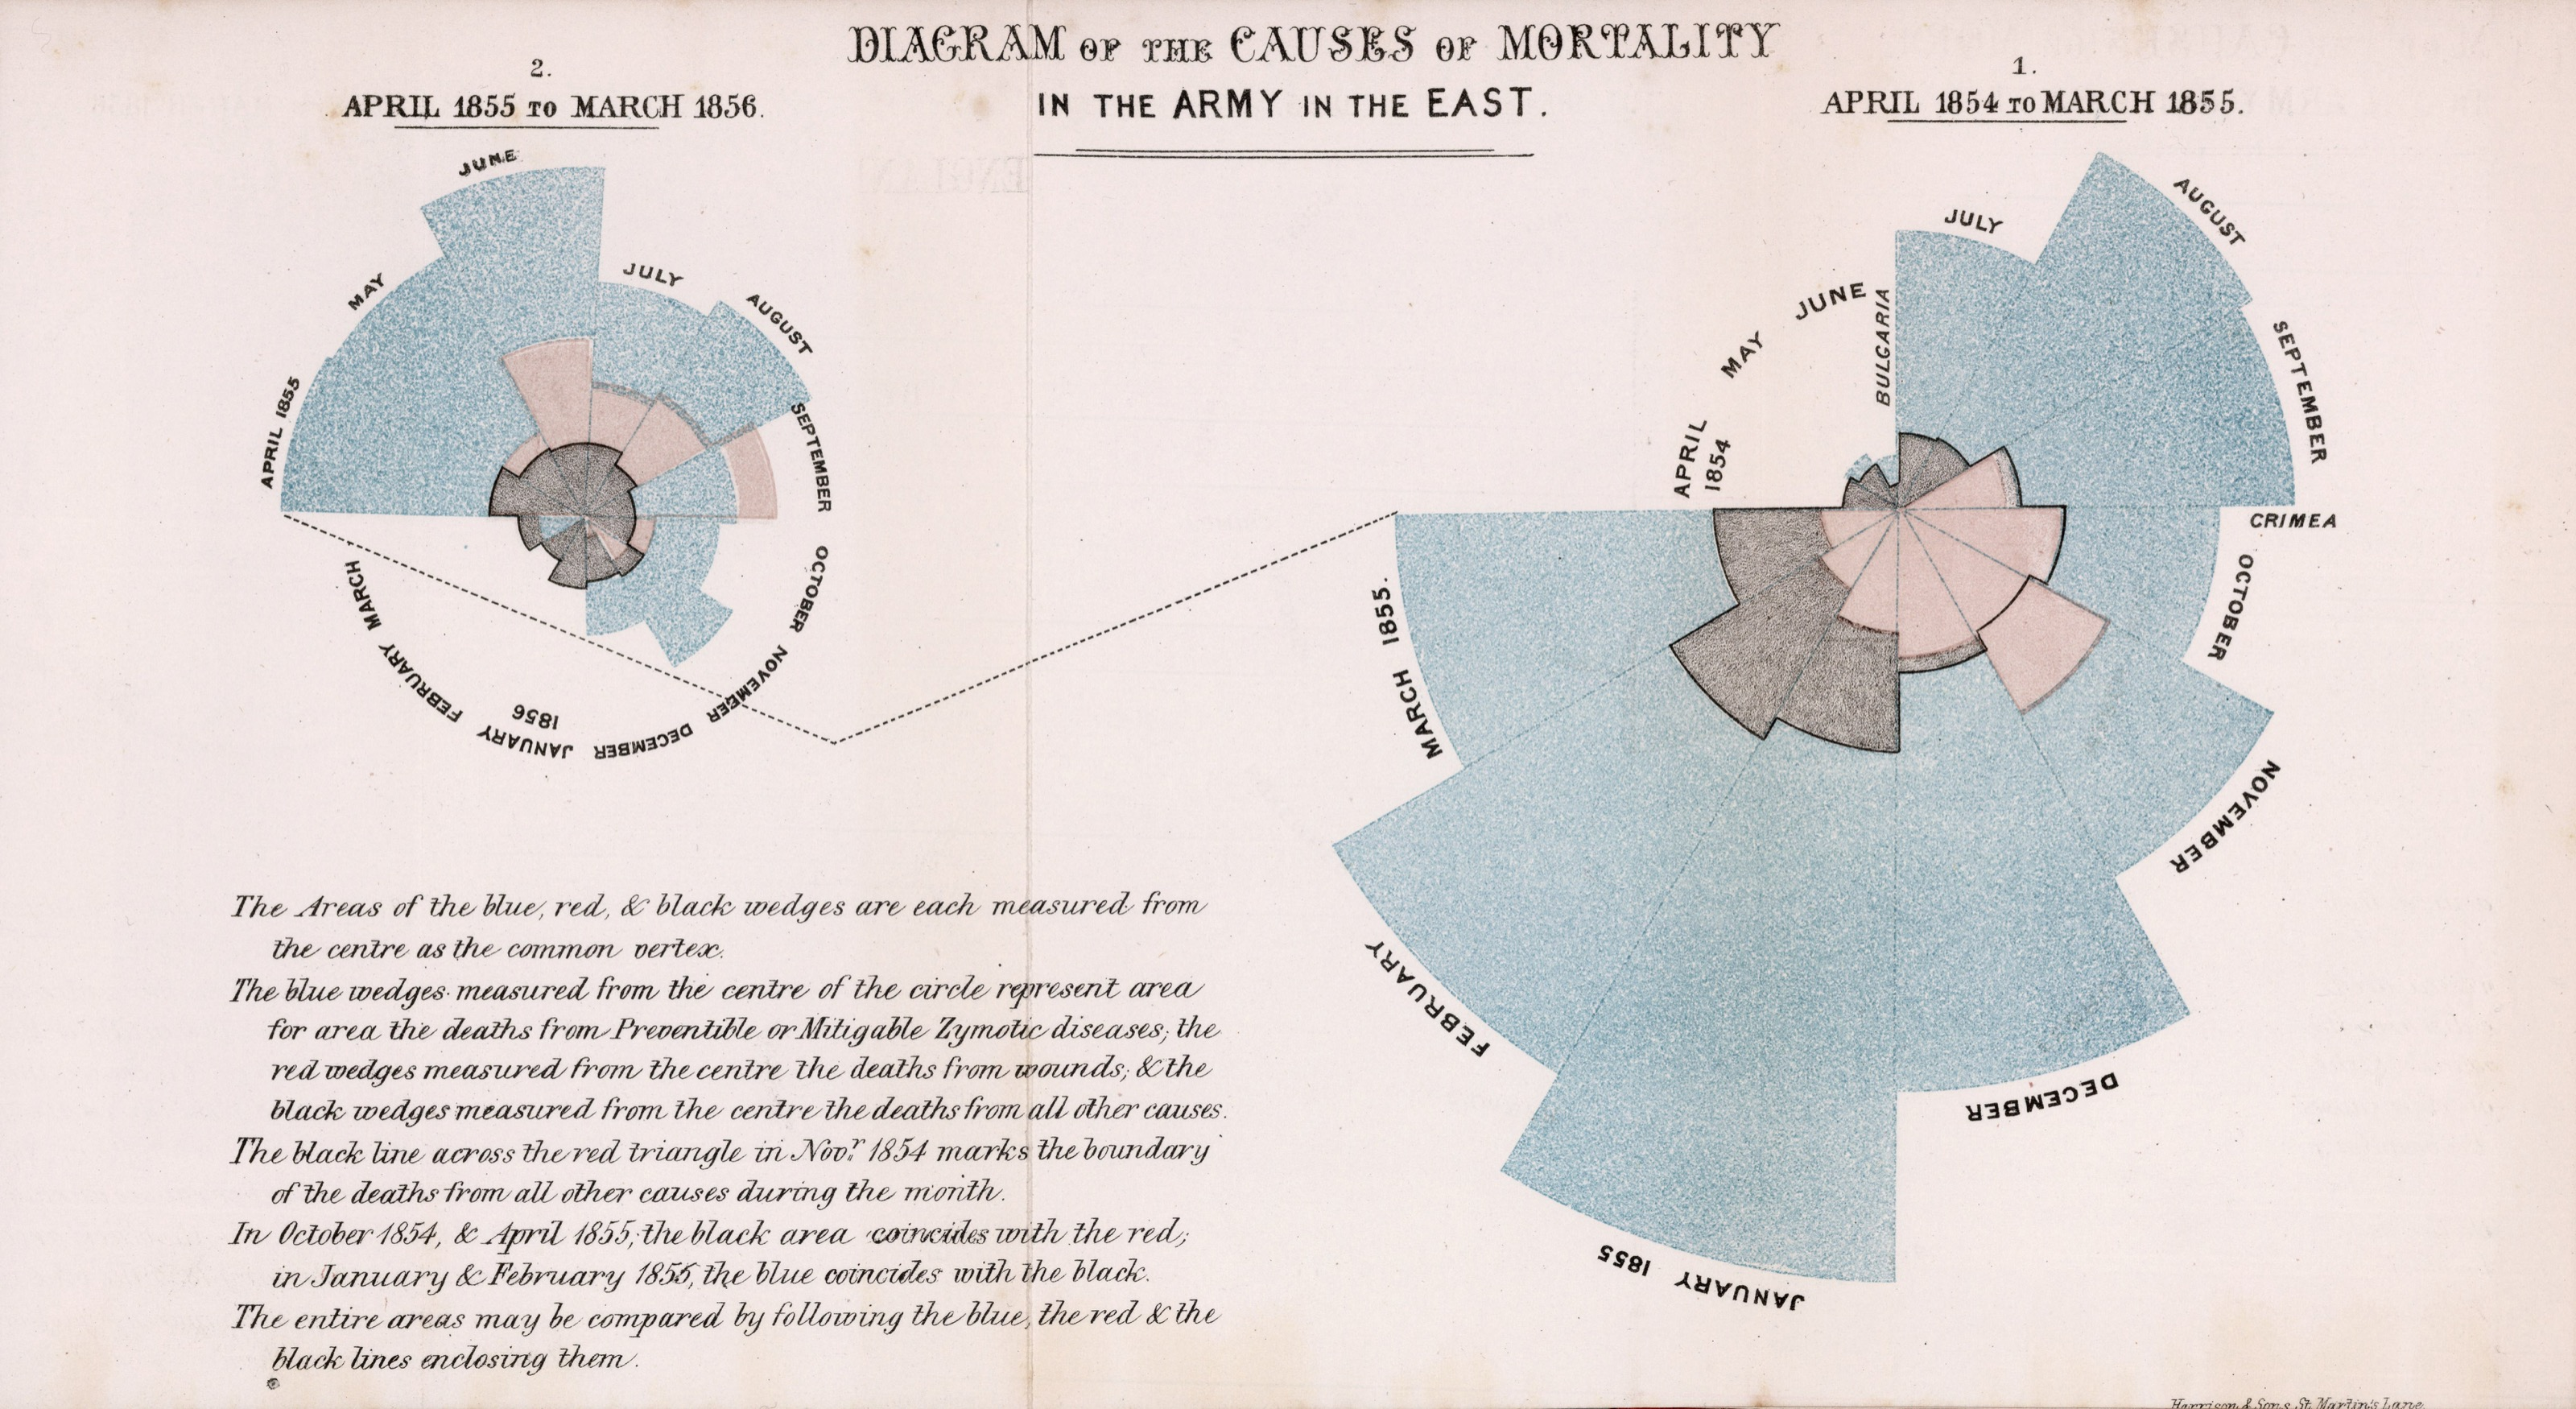
\includegraphics[width=\textwidth,height=0.52\textheight,keepaspectratio]{nightingale-original-1858.jpg}\\
      \credit{Florence Nightingale, \emph{Diagram of the causes of mortality in the army in the East}, 1858 (public domain).}
    \end{column}
    \begin{column}{0.34\textwidth}
      \small Write down, without discussion:
      \begin{itemize}
        \item what you \alert{see} — marks, colours, shapes;
        \item what you think it \alert{means};
        \item one thing you \alert{cannot tell} from the image alone.
      \end{itemize}
      \vspace{0.8em}
      \credit{Keep this page. We return to it at the end of class.}
    \end{column}
  \end{columns}
\end{frame}

% ---------- 3 · what did you write ----------
\begin{frame}{Two kinds of sentence}\framesubtitle{Debrief}
  \begin{itemize}
    \item \textbf{``The chart shows\,\dots''} — reserved for what is directly visible:\\
          blue wedges dwarf red ones; the wedges shrink after March 1855.
    \item \textbf{``This suggests\,\dots''} — interpretation:\\
          disease killed more soldiers than wounds; sanitation reforms worked.
  \end{itemize}
  \vspace{1em}
  Most of what a chart ``says'' is supplied by the reader.\\
  This class is about noticing when that happens — in you, and in a machine.
\end{frame}

% ---------- 4 · premise ----------
\kicker{The premise}{A chart is a claim about\\[0.1em] how the world is organised.}

\begin{frame}{Five decisions produce the claim}\framesubtitle{The premise}
  \begin{itemize}
    \item \textbf{Selection} — which data, which window, which denominator.
    \item \textbf{Encoding} — which visual channels carry which variables.
    \item \textbf{Comparison} — what is placed next to what.
    \item \textbf{Framing} — title, caption, annotation, baseline.
    \item \textbf{Omission} — everything left out, silently.
  \end{itemize}
  \vspace{0.8em}
  Opening question for every artefact this semester:\\
  \alert{what has the designer chosen to make visible — and what remains invisible?}
\end{frame}

% ---------- 5 · outcomes ----------
\begin{frame}{By the end of today}\framesubtitle{Learning outcomes}
  \begin{enumerate}
    \item Explain how selection, encoding and framing turn data into meaning.
    \item Separate observation from interpretation — in your own reading and in generated text.
    \item Explain why identical summary statistics can conceal different structures.
    \item Use an AI assistant to produce a chart, then verify every claim it makes.
    \item Apply representation and governance questions to a chart critique.
  \end{enumerate}
\end{frame}

% ---------- 6 · anscombe cold open ----------
\begin{frame}{Four datasets, one set of statistics}\framesubtitle{Cold open}
  \centering
  \begin{tabular}{lcccc}
    \toprule
     & I & II & III & IV \\
    \midrule
    mean of $x$        & 9.0 & 9.0 & 9.0 & 9.0 \\
    mean of $y$        & 7.50 & 7.50 & 7.50 & 7.50 \\
    variance of $x$    & 11.0 & 11.0 & 11.0 & 11.0 \\
    correlation        & 0.816 & 0.816 & 0.816 & 0.816 \\
    regression line    & \multicolumn{4}{c}{$y = 3.00 + 0.50\,x$} \\
    \bottomrule
  \end{tabular}
  \vspace{1.2em}

  \alert{Prediction:} will the four datasets look essentially the same when plotted?\\
  Write yes or no — and why — before the next slide.
\end{frame}

% ---------- 7 · anscombe reveal ----------
\begin{frame}[t]{Looking changes the conclusion}\framesubtitle{Anscombe's quartet, 1973}
  \centering
  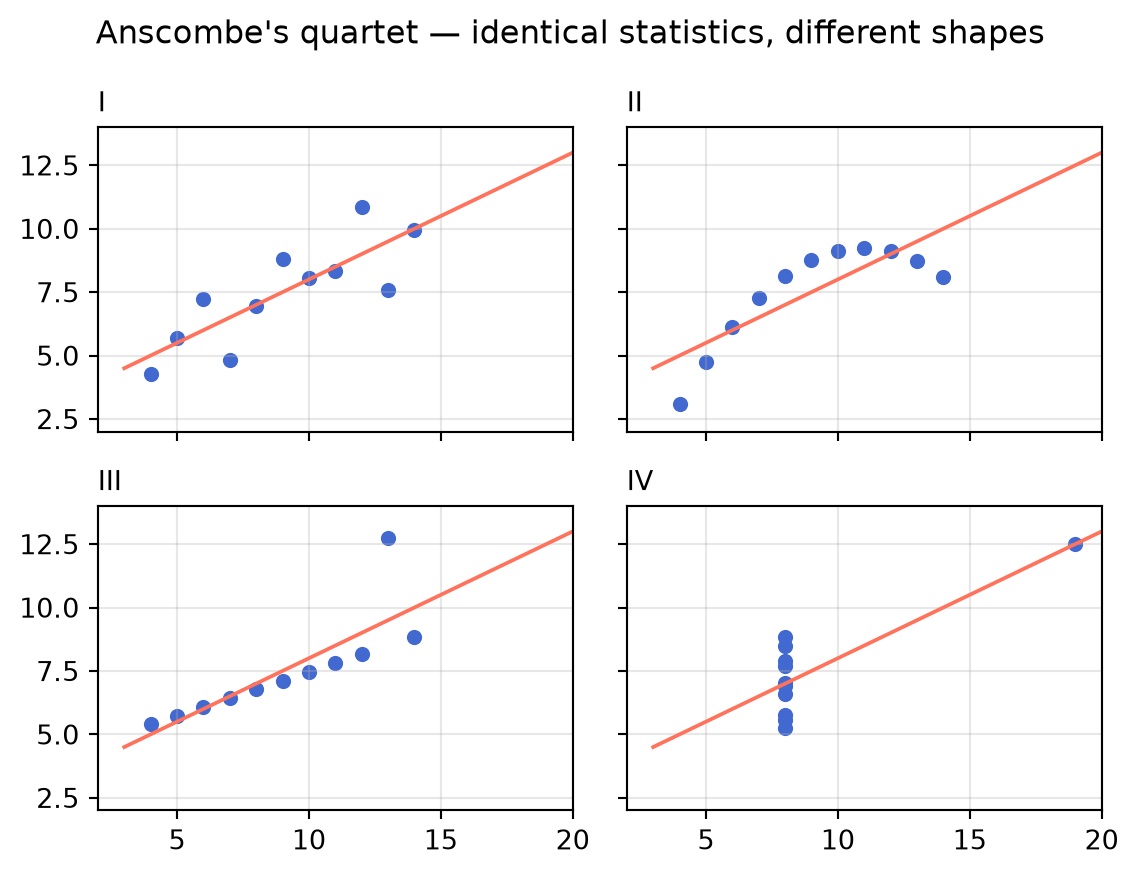
\includegraphics[height=0.58\textheight]{fig-anscombe-output-1.png}\\
  \credit{Course atlas reproduction of Anscombe (1973). A summary statistic is not a substitute for a picture.}
\end{frame}

% ---------- 8 · vocabulary ----------
\begin{frame}{The chain we will use all semester}\framesubtitle{Vocabulary}
  \centering
  {\large \textbf{data} \; $\rightarrow$ \; \textbf{encoding} \; $\rightarrow$ \; \textbf{observation} \; $\rightarrow$ \; \textbf{insight} \; $\rightarrow$ \; \textbf{narrative}}
  \vspace{1em}
  \begin{itemize}
    \item \textbf{data} — records of the world, already shaped by collection;
    \item \textbf{encoding} — the mapping of values onto marks and channels;
    \item \textbf{observation} — what any careful reader can see (``the chart shows'');
    \item \textbf{insight} — an interpretation that survives verification (``this suggests, because'');
    \item \textbf{narrative} — insights arranged to support a decision.
  \end{itemize}
  \vspace{0.6em}
  Every failure we study this semester is a broken link in this chain.
\end{frame}

% ---------- 9 · snow original ----------
\begin{frame}[t]{A picture can become an argument}\framesubtitle{Worked example · London, 1854}
  \begin{columns}[T]
    \begin{column}{0.60\textwidth}
      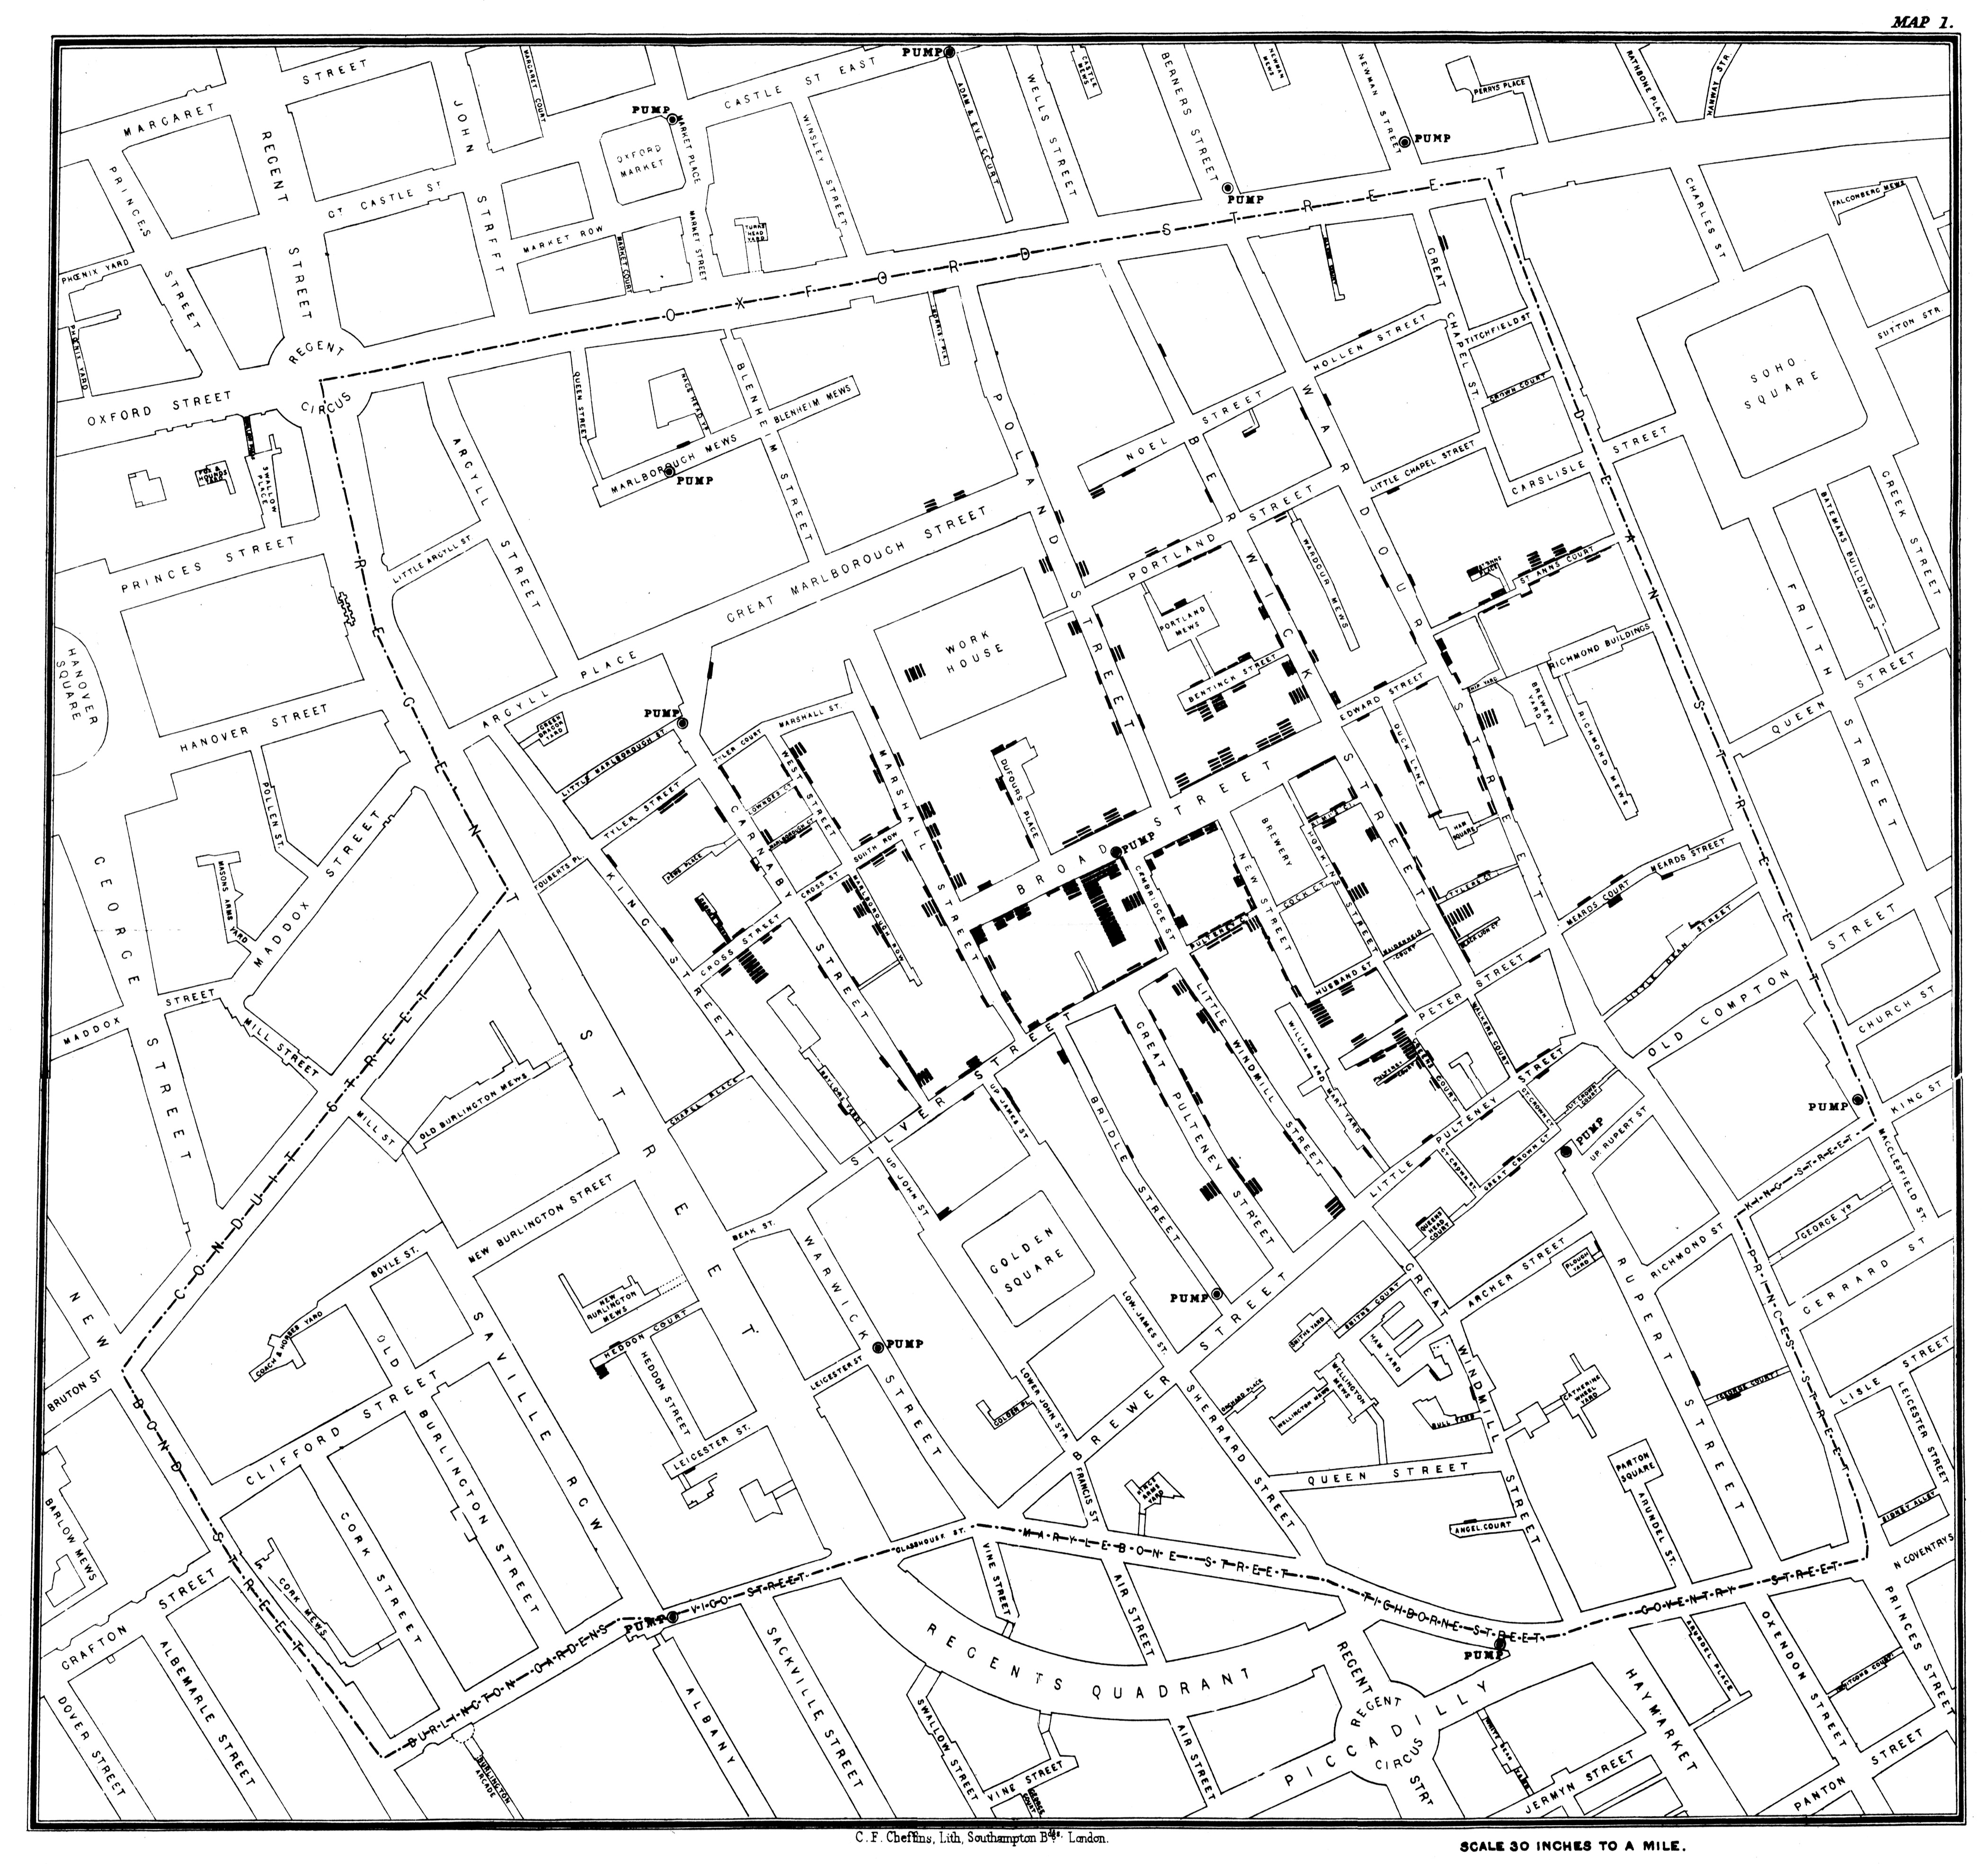
\includegraphics[width=\textwidth,height=0.56\textheight,keepaspectratio]{snow-original-1854.jpg}\\
      \credit{John Snow's map of cholera deaths, Soho, 1854; published in \emph{On the Mode of Communication of Cholera}, 1855. Public domain.}
    \end{column}
    \begin{column}{0.36\textwidth}
      \small Each black bar: one death, stacked at an address.\\[0.8em]
      Read it with the chain:
      \begin{itemize}
        \item what is the \alert{encoding}?
        \item what is the strongest \alert{observation}?
        \item what \alert{insight} is Snow selling?
      \end{itemize}
    \end{column}
  \end{columns}
\end{frame}

% ---------- 10 · snow pattern vs claim ----------
\begin{frame}[t]{Pattern, inference, and the missing evidence}\framesubtitle{Worked example · London, 1854}
  \begin{columns}[T]
    \begin{column}{0.48\textwidth}
      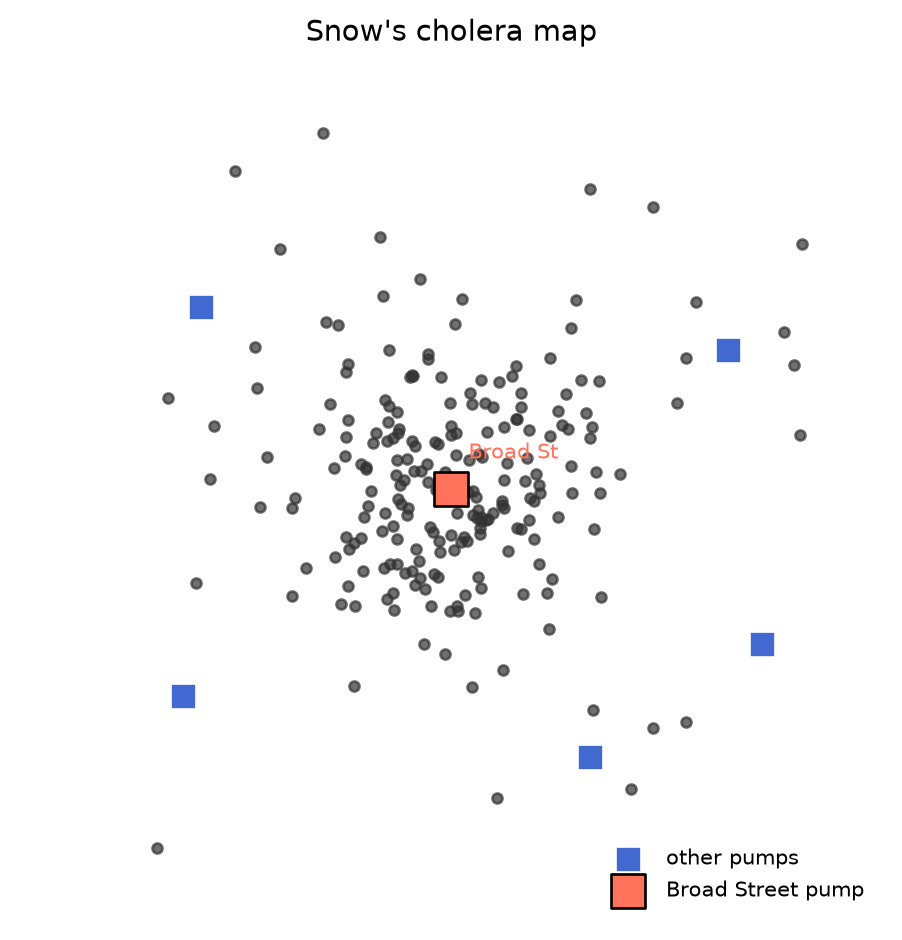
\includegraphics[width=\textwidth]{fig-snow-output-1.png}\\
      \credit{Course atlas reproduction: deaths cluster on the Broad Street pump.}
    \end{column}
    \begin{column}{0.48\textwidth}
      \small
      \begin{itemize}
        \item \textbf{Pattern:} deaths cluster around one pump. Visible.
        \item \textbf{Inference:} the water is the vehicle. Not visible — argued.
        \item \textbf{Causal evidence} came from elsewhere: the brewery workers who drank beer; the workhouse with its own well; deaths that stopped after the handle came off.
      \end{itemize}
      \vspace{0.5em}
      The map did not prove the theory.\\ It made the theory \alert{impossible to ignore}.
    \end{column}
  \end{columns}
\end{frame}

% ---------- 11 · six mechanisms ----------
\begin{frame}{Six ways a true chart misleads}\framesubtitle{How charts lie}
  Every number checked, every label true — and the impression still wrong.
  \begin{columns}[T]
    \begin{column}{0.48\textwidth}
      \begin{itemize}
        \item truncated or missing baseline
        \item cherry-picked time window
        \item dual axes tuned to a story
      \end{itemize}
    \end{column}
    \begin{column}{0.48\textwidth}
      \begin{itemize}
        \item area standing in for value
        \item binning and smoothing choices
        \item omitted denominators
      \end{itemize}
    \end{column}
  \end{columns}
  \vspace{0.8em}
  \credit{After Cairo, \emph{How Charts Lie} (required reading, selected chapter).}
\end{frame}

% ---------- 12 · window ----------
\begin{frame}[t]{The window is part of the claim}\framesubtitle{How charts lie}
  \small Crop either one to 1998–2012 and you can sell a pause. The axis window is an editorial decision.
  \vspace{0.5em}
  \begin{columns}[T]
    \begin{column}{0.48\textwidth}
      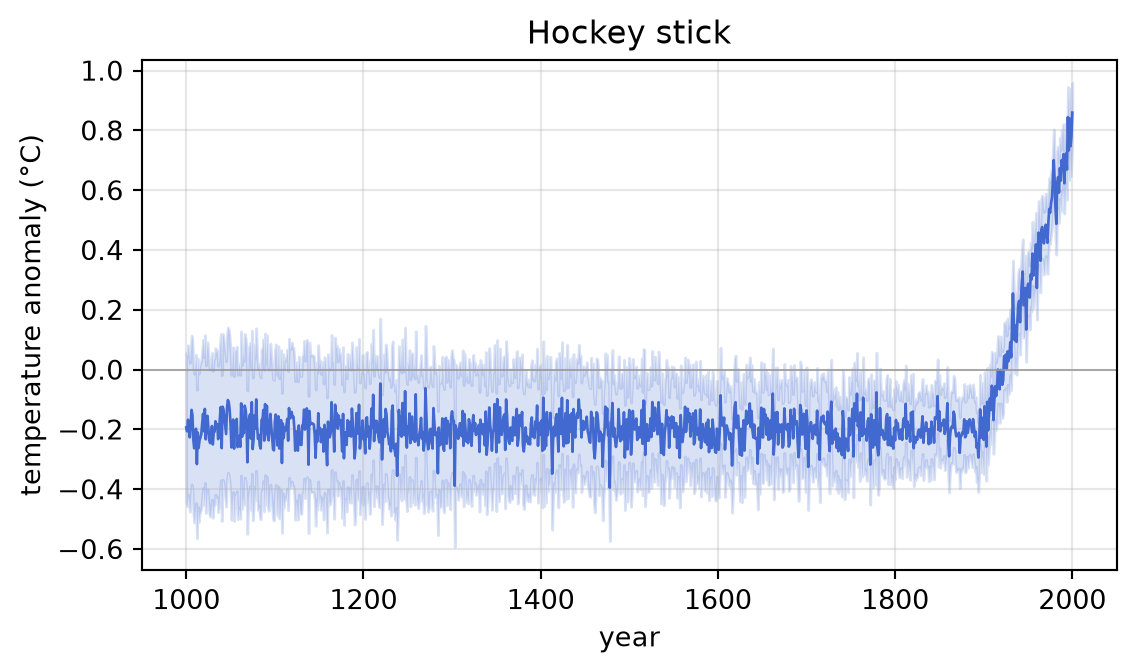
\includegraphics[width=\textwidth,height=0.5\textheight,keepaspectratio]{fig-hockeystick-output-1.png}\\
      \credit{Course atlas: the hockey stick — context makes the rise the story.}
    \end{column}
    \begin{column}{0.48\textwidth}
      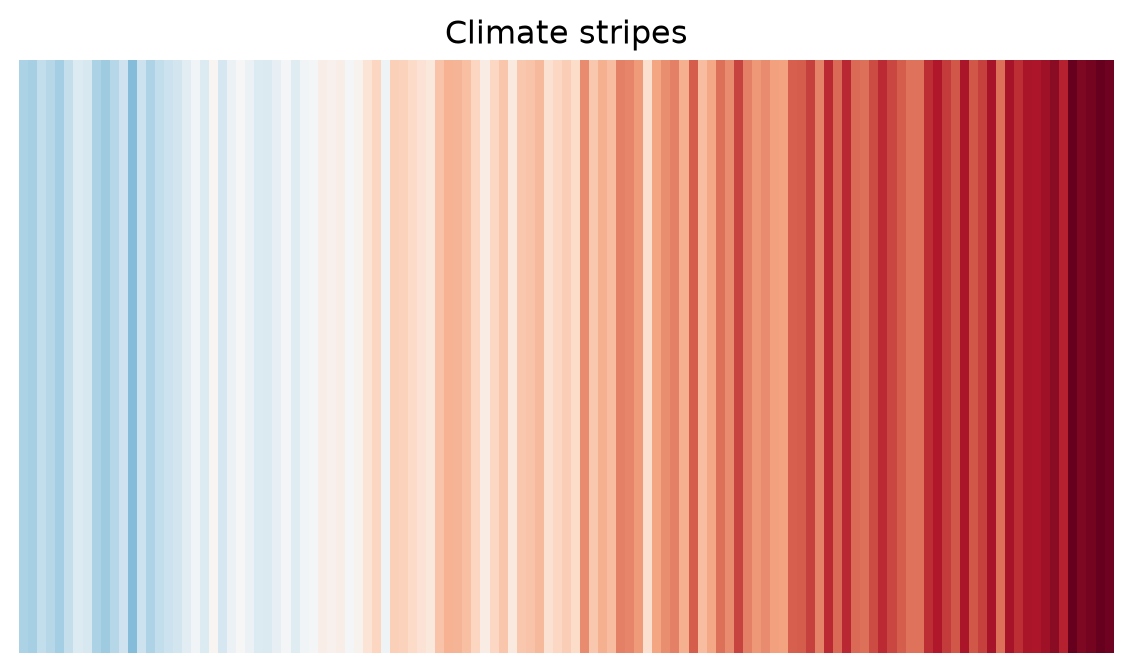
\includegraphics[width=\textwidth,height=0.5\textheight,keepaspectratio]{fig-climatestripes-output-1.png}\\
      \credit{Course atlas: climate stripes — the same claim, at a glance.}
    \end{column}
  \end{columns}
\end{frame}

% ---------- 13 · AI section ----------
\kicker{Visualisation + AI}{Fluent interpretation is not\\[0.1em] valid interpretation.}

\begin{frame}{What the assistant does well — and doesn't}\framesubtitle{Visualisation + AI}
  \begin{itemize}
    \item An AI system can describe a pattern \alert{confidently} without checking whether the data supports the claim.
    \item Generated text is optimised to read well. Reading well and being right are different properties.
    \item The failure mode is not usually a wrong number — it is an \alert{unsupported claim} delivered in a supported tone.
  \end{itemize}
  \vspace{0.8em}
  Your job is not to avoid the assistant. It is to \textbf{own the verification}.
\end{frame}

% ---------- 14 · ladder ----------
\begin{frame}{The verification ladder}\framesubtitle{For any generated chart or interpretation}
  \begin{enumerate}
    \item \textbf{Source} — what data was actually used? Can you point to it?
    \item \textbf{Transformation} — what was filtered, aggregated, reshaped? Check counts and types.
    \item \textbf{Visibility} — is each claimed pattern actually visible in the plotted data?
    \item \textbf{Support} — classify each claim: \alert{supported / plausible but unverified / unsupported / contradicted}.
    \item \textbf{Disclosure} — record what the tool contributed and what remains unverified.
  \end{enumerate}
  \vspace{0.6em}
  This ladder is the spine of the notebook today — and of Assessment 1, Part C.
\end{frame}

% ---------- 15 · uncertainty ----------
\begin{frame}[t]{Uncertainty drawn rather than suppressed}\framesubtitle{Visualisation + AI}
  \centering
  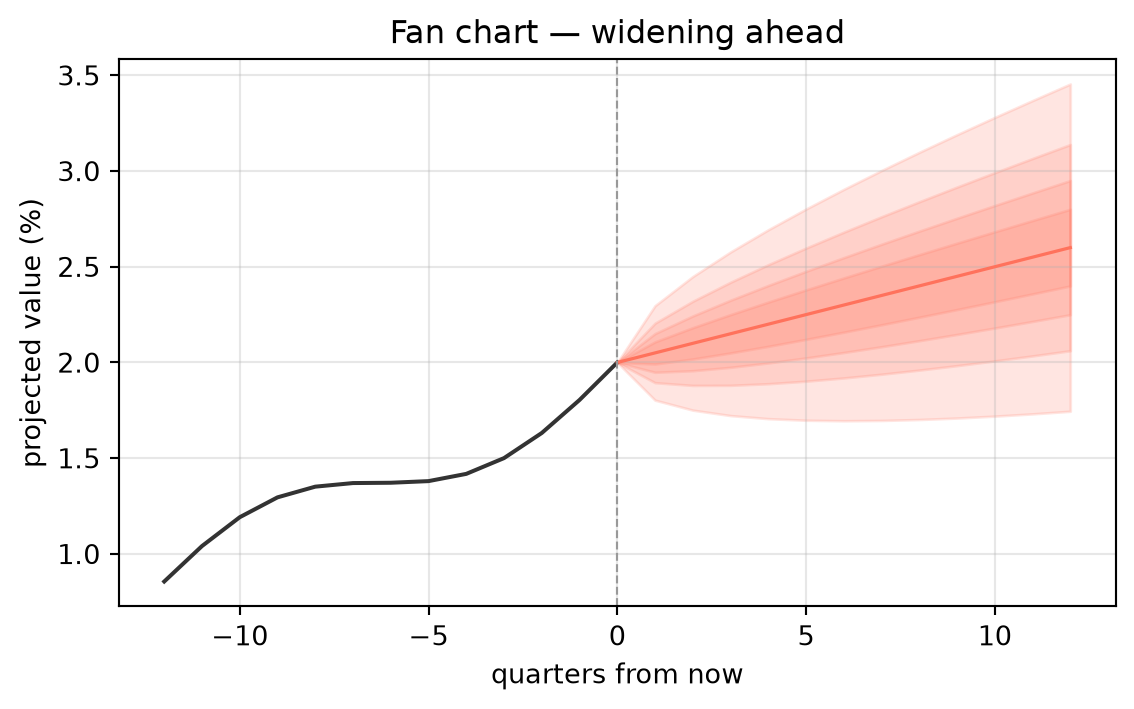
\includegraphics[height=0.55\textheight]{fig-fanchart-output-1.png}\\
  \credit{Course atlas: a fan chart admits what it does not know. Generated interpretations rarely volunteer this — you must ask.}
\end{frame}

% ---------- 16 · think pair share ----------
\begin{frame}{Think · pair · share}\framesubtitle{5 minutes solo · 5 in pairs · 5 as a room}
  Find a chart published \alert{this week} — news, social, a report.
  \begin{itemize}
    \item What claim does it make?
    \item Which of the six mechanisms should worry you?
    \item What would you need to verify before repeating its claim?
  \end{itemize}
  \vspace{0.8em}
  \textbf{Keep the chart.} It may become your Assessment 1 artefact.
\end{frame}

% ---------- 17 · break ----------
\kicker{Break · 10 minutes}{When we return:\\[0.1em] who owns the data, then the lab.}

% ---------- 18 · aiatsis ----------
\begin{frame}[t]{Representation is also governance}\framesubtitle{Acknowledgement of Country}
  \begin{columns}[T]
    \begin{column}{0.60\textwidth}
      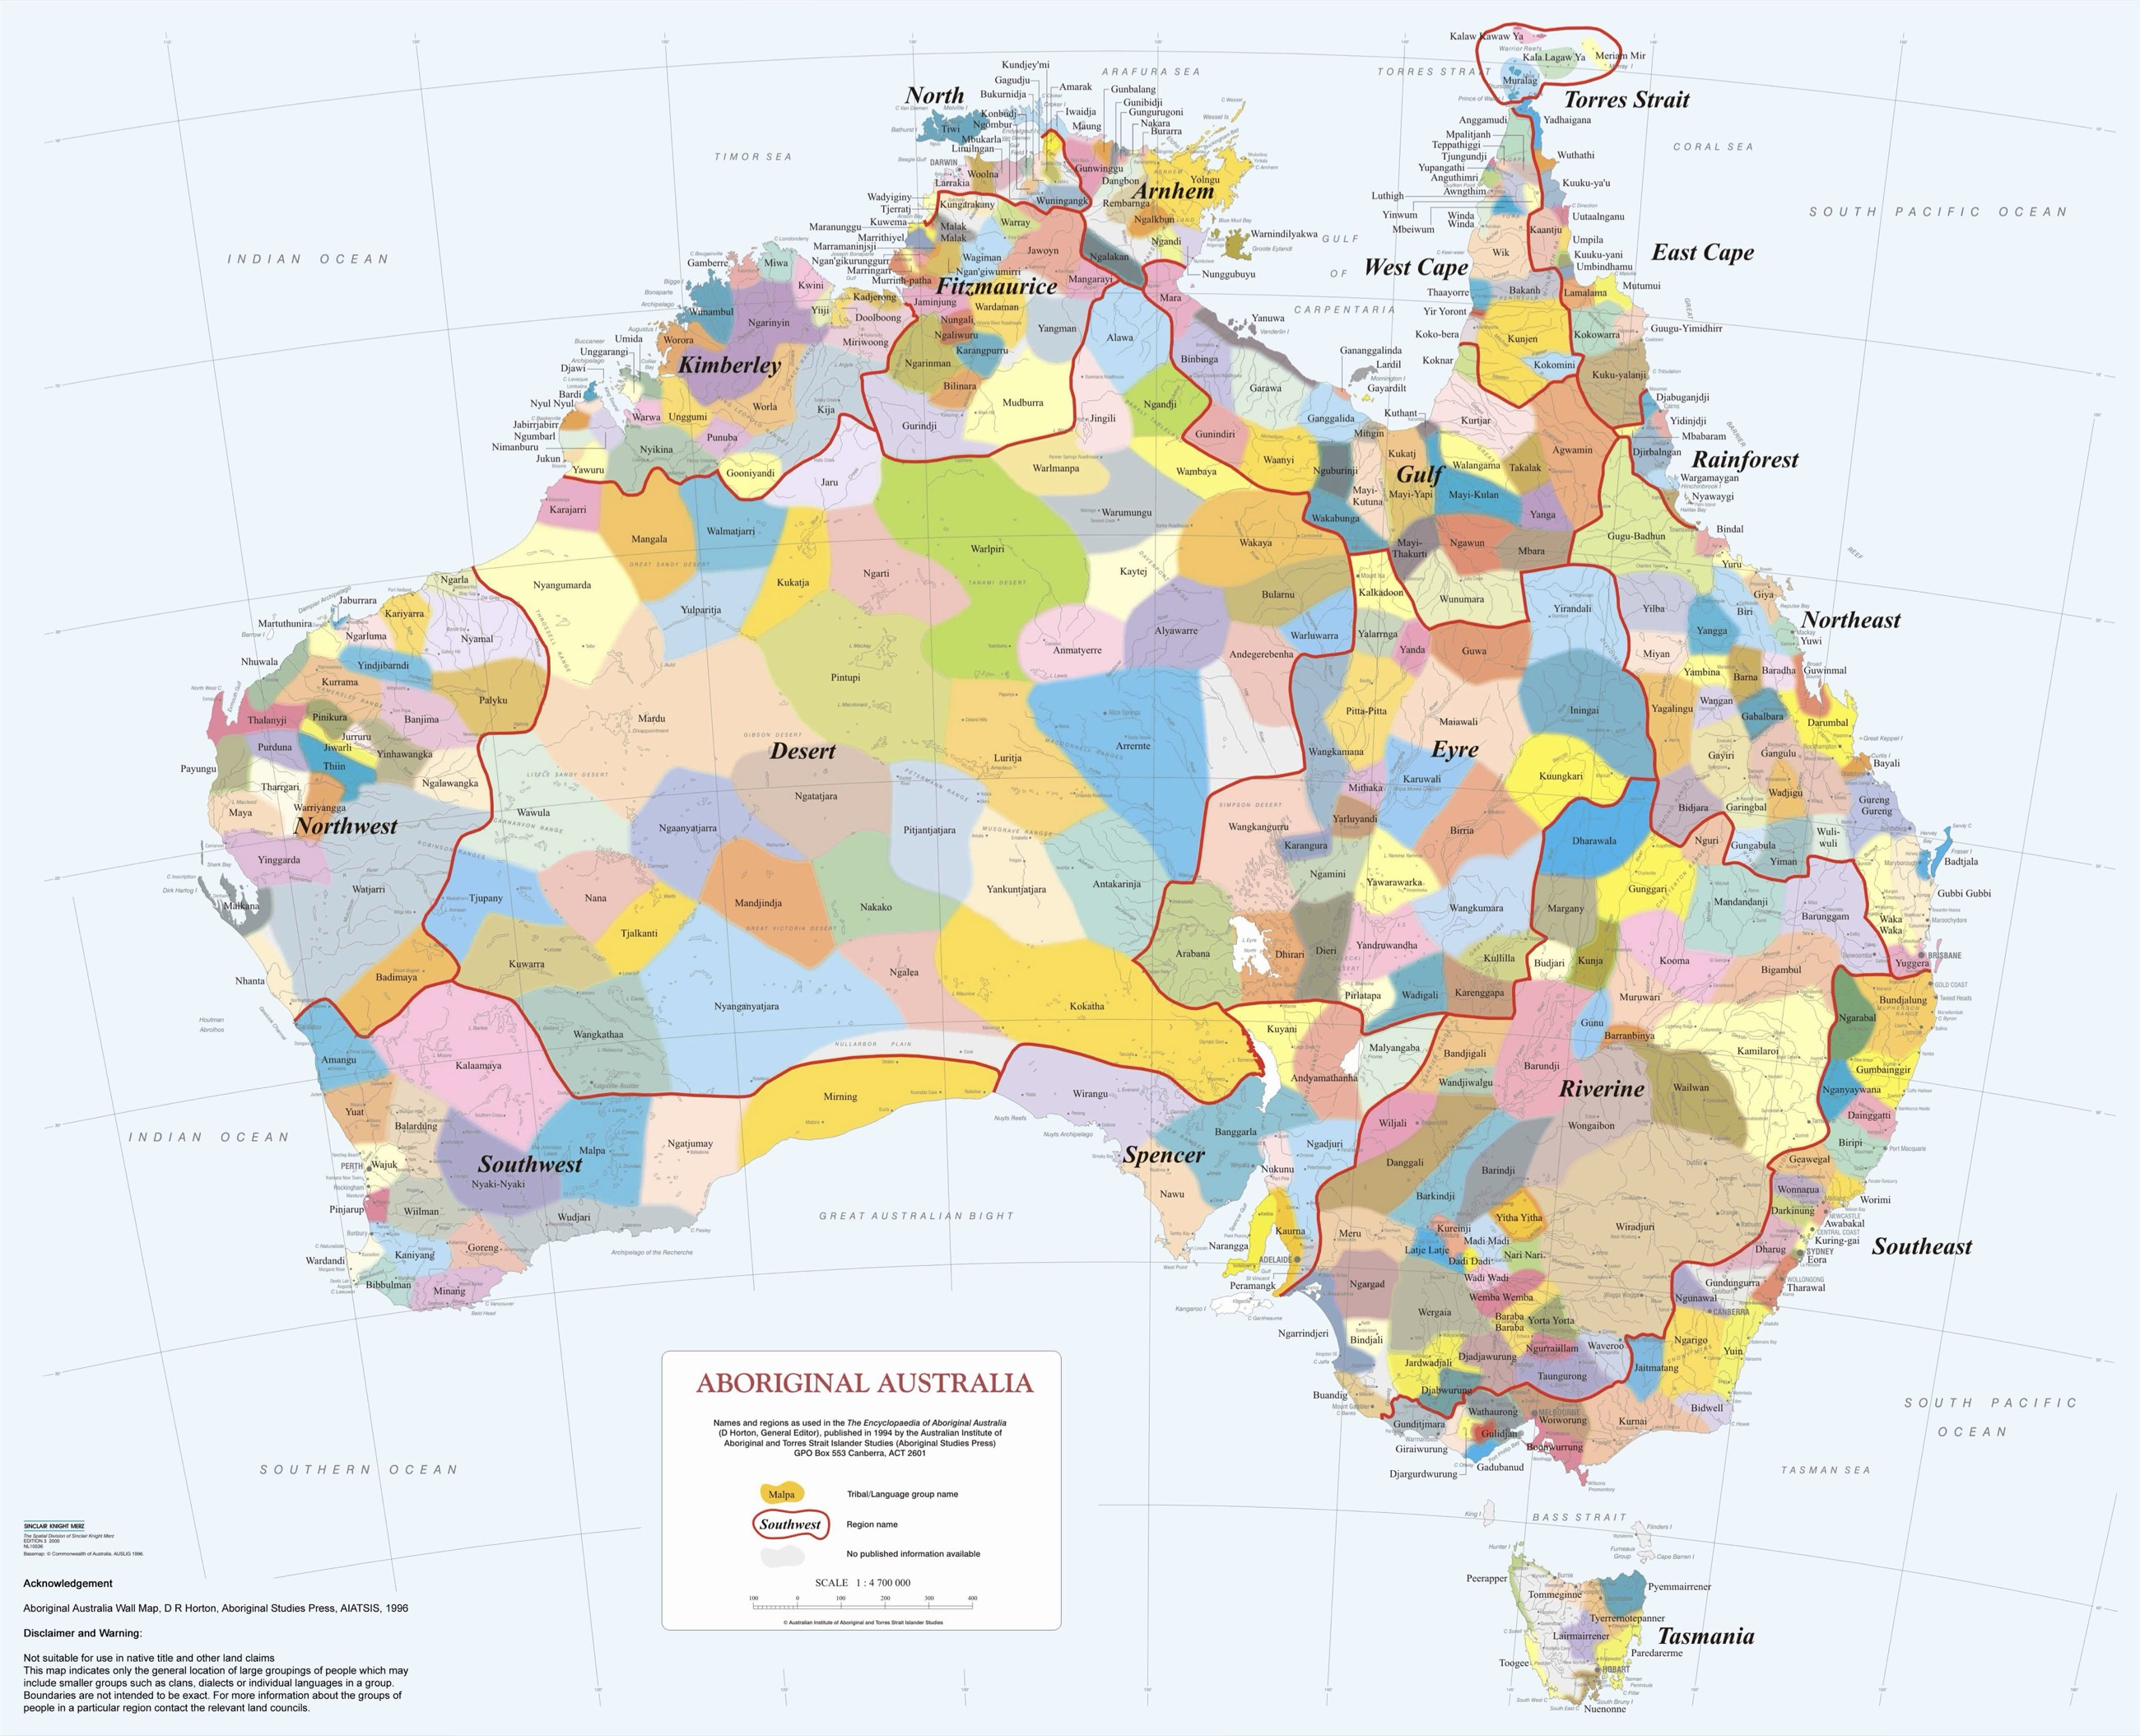
\includegraphics[width=\textwidth,height=0.56\textheight,keepaspectratio]{aiatsis-map.jpg}\\
      \credit{Aboriginal Australia Wall Map, D R Horton, © Aboriginal Studies Press, AIATSIS, 1996.}
    \end{column}
    \begin{column}{0.36\textwidth}
      \small This class was written and is taught on Aboriginal land.\\[0.6em]
      More than 250 language, social and nation groups on one sheet — a claim that the land was never empty.\\[0.6em]
      Its boundaries are deliberately soft: a general guide, contested in places, and explicitly not evidence for legal claims.
    \end{column}
  \end{columns}
\end{frame}

% ---------- 19 · governance questions ----------
\begin{frame}{Four questions that outrank aesthetics}\framesubtitle{Indigenous Data Sovereignty}
  \begin{itemize}
    \item Who is \textbf{represented} in this data — and who was consulted?
    \item Who \textbf{benefits} from this visualisation?
    \item Who could be \textbf{harmed or misled} by it?
    \item What limitation \textbf{must be disclosed} before it circulates?
  \end{itemize}
  \vspace{0.8em}
  \credit{Required reading: Maiam nayri Wingara \& AIGI, \emph{Indigenous Data Sovereignty Communique}. These four questions appear in every critique this semester, including Assessment 1.}
\end{frame}

% ---------- 20 · lab ----------
\begin{frame}{Notebook lab · 45 minutes}\framesubtitle{seeing\_data\_lab.ipynb}
  \begin{enumerate}
    \item \textbf{Anscombe} — summary statistics vs the picture.
    \item \textbf{Generate and verify} — assistant-drawn chart of the transport dataset, then the checks: rows, types, missing values, totals.
    \item \textbf{Claim audit} — a generated interpretation, every sentence classified: supported / plausible but unverified / unsupported / contradicted.
  \end{enumerate}
  \vspace{0.6em}
  The contract: \alert{predict} before you generate · give the assistant a \alert{bounded task} ·
  \alert{verify} before you accept · \alert{disclose} at the end.\\[0.4em]
  \credit{Blocked on syntax? Ask for the starter notebook — that is what it is for.}
\end{frame}

% ---------- 21 · studio ----------
\begin{frame}{Studio · Critique and Repair · 25 minutes}\framesubtitle{Activity sheet in activities/}
  \begin{itemize}
    \item \textbf{Read} the assigned artefact: main claim, audience, what is directly visible.
    \item \textbf{Test} the design: encodings, easy comparisons, what is aggregated or hidden.
    \item \textbf{Verify and repair}: what you would check, an alternative view, a repaired caption.
    \item \textbf{Responsibility}: who benefits — and who carries the cost if it is wrong?
  \end{itemize}
  \vspace{0.6em}
  Ten minutes solo, ten with a partner, five to revise.
\end{frame}

% ---------- 22 · pair exchange ----------
\begin{frame}{Pair exchange · the Critique 1 frame}\framesubtitle{Rehearsal for Assessment 1}
  Swap artefacts: one \textbf{human-made chart}, one \textbf{AI-generated interpretation}.
  \begin{itemize}
    \item Same questions for both: claim, audience, task, comparison, omission.
    \item Then the AI-specific one: \alert{which claims would survive the ladder?}
  \end{itemize}
  \vspace{0.8em}
  This is exactly Assessment 1, Parts A and C, at rehearsal scale:\\
  Part A critique (supervised, in studio) · Part B redesign $\times$3 (next class) · Part C claim audit.
\end{frame}

% ---------- 23 · closing ----------
\begin{frame}{Close the loop}\framesubtitle{Exit ticket}
  Look back at your silent reading of the Nightingale diagram.\\
  \alert{Which of your sentences were observations? Which were interpretations?}
  \vspace{0.8em}
  \begin{itemize}
    \item One design decision I made today:
    \item One risk or limitation I noticed:
    \item One thing I need to verify before next class:
  \end{itemize}
  \vspace{0.8em}
  \credit{Diagnostic quiz on Canvas after class — open book, closed assistant, ungraded. It calibrates the course, not your mark. Next class: Choosing Visual Forms — what visual task are we performing?}
\end{frame}

% ---------- 24 · credits ----------
\begin{frame}{Image credits and reading}\framesubtitle{Colophon}
  \small
  \begin{itemize}
    \item Nightingale (1858) and Snow (1855) images: public domain, via Wikimedia Commons.
    \item AIATSIS map: © Aboriginal Studies Press, AIATSIS and Auslig/Sinclair, Knight, Merz, 1996. Reproduced with attribution for teaching; view the official copy at aiatsis.gov.au.
    \item All other figures: course atlas reproductions (\emph{How the World Is Organised}), generated from data.
  \end{itemize}
  \vspace{0.6em}
  Required reading: Cairo, \emph{How Charts Lie} (ch.); D'Ignazio \& Klein, \emph{Data Feminism} (ch.); Maiam nayri Wingara \& AIGI, \emph{Indigenous Data Sovereignty Communique}.
\end{frame}

\end{document}
